	\subsection{Paso 5: Límite del Sistema, Declaración de Visión, Ocho Perspectivas de Contexto y Mapa Conceptual}
\subsubsection{a) Definición del Límite del Sistema y Entidades Externas (Mín. 5 Interfaces)}
Siguiendo la metodología de Pohl (2025) \cite{pohl2025} e ISO/IEC/IEEE 29148:2018 \cite{ieee29148}, el límite de la Plataforma de Ventas abarca internamente los procesos de gestión de inventario eléctrico, facturación comercial, preparación de consultas contextualizadas al catálogo y auditoría de operaciones. Quedan fuera del límite del sistema —interactuando exclusivamente mediante interfaces bien definidas— las cinco entidades externas detalladas en la Tabla \ref{tab:entidades_externas}:
\begin{table}[htbp]
	\centering
	\scriptsize
	\caption{Especificación de Entidades Externas e Interfaces en el Límite del Sistema del PFC \cite{ieee29148, pohl2025}}
	\label{tab:entidades_externas}
	\begin{tabularx}{\textwidth}{l >{\raggedright\arraybackslash}p{0.18\textwidth} Y >{\raggedright\arraybackslash}p{0.18\textwidth} >{\raggedright\arraybackslash}p{0.18\textwidth}}
		\toprule
		\textbf{ID} & \textbf{Entidad Externa} & \textbf{Tipo y Estructura Lógica de Datos Intercambiados} & \textbf{Protocolo / Estándar de Interfaz} & \textbf{Frecuencia Operativa} \\
		\midrule
		EXT-01 & Servicio Externo de Inferencia de IA & \textbf{Entrada/Salida:} Consulta técnica del suministro eléctrico con parámetros de catálogo disponible y respuesta estructurada con 3 sugerencias y justificación de equivalencia eléctrica. & Protocolo seguro de transferencia web sobre TLS 1.2+ (Mensajes de texto estructurados UTF-8) & Bajo demanda en mostrador ($\approx 80\text{--}150$ consultas/día). \\
		\midrule
		EXT-02 & Plataforma de Comprobantes Electrónicos del SRI & \textbf{Entrada/Salida:} Comprobante electrónico firmado digitalmente y mensaje oficial de recepción/autorización tributaria con clave de acceso de 49 dígitos. & Servicios web gubernamentales sobre canal cifrado TLS 1.2+ (Esquema estándar SRI) & Tiempo real por cada venta facturada ($\approx 200\text{--}400$ tx/día). \\
		\midrule
		EXT-03 & Pasarela de Cobros Bancarios / Electrónicos & \textbf{Entrada/Salida:} Solicitud de cobro (monto total, desglose de impuestos, identificador de transacción) y código de aprobación o rechazo financiero. & Interfaz de comunicación financiera cifrada sobre red TCP/IP & Por cada cobro con tarjeta o pago electrónico ($\approx 60\text{--}120$ tx/día). \\
		\midrule
		EXT-04 & Dispositivo Lector Óptico de Código de Barras & \textbf{Entrada hacia el Sistema:} Secuencia alfanumérica correspondiente a simbologías estándar EAN-13, EAN-8 y Code-128 de suministros eléctricos con carácter de fin de línea. & Interfaz estándar de dispositivo de entrada humana (USB HID) & Continua de alta frecuencia ($\ge 30$ lecturas/min en hora pico). \\
		\midrule
		EXT-05 & Impresora Térmica de Comprobantes (80 mm) & \textbf{Salida desde el Sistema:} Flujo de datos de impresión con detalle del comprobante de venta, desglose tributario y señal de corte de papel. & Estándar de comandos de impresión térmica de punto de venta (USB / Red local) & Inmediata al cierre de cada venta ($\approx 200\text{--}400$ impresiones/día). \\
		\bottomrule
	\end{tabularx}
\end{table}
\subsubsection{b) Declaración de Visión del Producto en Formato de Geoffrey Moore}
Aplicando la plantilla canónica de posicionamiento estratégico de Geoffrey A. Moore \cite{moore2014}, adoptada en la ingeniería de requisitos por Wiegers \& Beatty \cite{wiegers2013}, se formula la declaración de visión oficial del Proyecto Fin de Curso:
\begin{quote}
	\textbf{Declaración de Visión (Formato Moore \cite{moore2014}):} \\
	\textit{``\textbf{Para} los cajeros, administradores y propietarios de almacenes comercializadores de suministros eléctricos en Quevedo \textbf{que} enfrentan cuellos de botella en la facturación en horas pico y pérdida de ventas por falta de conocimientos electrotécnicos para recomendar componentes compatibles o sustitutos, \textbf{la} Plataforma de Ventas con Módulo de Recomendación basado en Inteligencia Artificial \textbf{es un} sistema de información transaccional e inteligente de gestión comercial \textbf{que} agiliza el cobro por teclado y lector óptico, automatiza la emisión de comprobantes electrónicos hacia el SRI y sugiere en menos de 3 segundos tres productos eléctricos técnicamente equivalentes con existencias reales verificadas en el inventario. \textbf{A diferencia de} los sistemas de facturación tradicionales o la consulta manual de catálogos impresos, \textbf{nuestro producto} integra el control de inventario en tiempo real con asistencia técnica inteligente acotada al stock disponible del local, garantizando recomendaciones seguras en mostrador sin riesgo de ofrecer artículos agotados.''}
\end{quote}
\subsubsection{c) Análisis Exhaustivo de las Ocho Perspectivas de Contexto de Pohl Aplicadas al PFC}
Conforme al Paso 5c de la Guía de Práctica y al marco teórico de Klaus Pohl (2025) \cite{pohl2025}, en la Tabla \ref{tab:ocho_perspectivas} se evalúan las ocho perspectivas de contexto sobre el sistema del PFC, formulando para cada una (a) \textbf{tres preguntas clave de indagación} (24 preguntas en total) y (b) \textbf{dos requisitos o restricciones concretas que emergen} de dicho análisis (16 requisitos/restricciones emergentes en total, libres de tecnologías de diseño).
\begin{table}[htbp]
	\centering
	\scriptsize
	\caption{Aplicación de las Ocho Perspectivas de Contexto de Pohl (2025) \cite{pohl2025} al Sistema del PFC}
	\label{tab:ocho_perspectivas}
	\begin{tabularx}{\textwidth}{>{\raggedright\arraybackslash}p{0.18\textwidth} Y Y}
		\toprule
		\textbf{Perspectiva de Contexto \cite{pohl2025}} & \textbf{(a) Tres Preguntas Clave de Elicitación Contextual} & \textbf{(b) Dos Requisitos / Restricciones que Emergen para el PFC} \\
		\midrule
		\textbf{1. Perspectiva de Sujeto (Datos y Dominio)} &
		1. ¿Qué atributos técnicos definen la compatibilidad eléctrica entre dos componentes (voltaje nominal, amperaje, curva de disparo, calibre, número de polos)? \newline
		2. ¿Cómo se clasifican las relaciones de equivalencia e intercambiabilidad en el catálogo de suministros? \newline
		3. ¿Qué volumen histórico de comprobantes y movimientos de inventario debe conservarse? &
		\textbf{Emergente 1.1:} El catálogo del sistema deberá registrar atributos técnicos normalizados por cada artículo eléctrico (tensión, corriente nominal, capacidad de ruptura y normativa técnica) para fundamentar las sugerencias de equivalencia. \newline
		\textbf{Emergente 1.2:} Toda recomendación generada estará restringida estrictamente a artículos con saldo disponible mayor a cero en la bodega local (ref. REQ-04). \\
		\midrule
		\textbf{2. Perspectiva de Uso (Actores y Flujos)} &
		1. ¿Cuál es el nivel de destreza operativa y de conocimientos en electricidad de los cajeros actuales del local en Quevedo? \newline
		2. ¿Con qué frecuencia un comprador solicita asesoría de reemplazo técnico frente a una compra directa? \newline
		3. ¿Qué acciones repetitivas generan mayor fatiga o errores de digitación en la jornada laboral? &
		\textbf{Emergente 2.1:} La interfaz de facturación permitirá operar el flujo completo mediante atajos de teclado (F1--F12) y posicionamiento automático en el campo de lectura óptica (ref. REQ-03). \newline
		\textbf{Emergente 2.2:} Las 3 sugerencias del módulo de IA mostrarán en lenguaje claro la justificación de compatibilidad eléctrica y la diferencia de precio unitario. \\
		\midrule
		\textbf{3. Perspectiva de Entorno TI (Infraestructura)} &
		1. ¿Bajo qué condiciones de conectividad y equipamiento operan actualmente las terminales de caja del almacén? \newline
		2. ¿Cómo debe comportarse la Plataforma de Ventas si se interrumpe la conexión externa con el servicio de IA o con el SRI? \newline
		3. ¿Qué periféricos físicos de mostrador deben interactuar con el sistema? &
		\textbf{Emergente 3.1:} Si el servicio externo de IA supera los $3.0\text{ s}$ de respuesta, el sistema conmutará automáticamente a una búsqueda local determinista por subcategoría eléctrica en $\le 200\text{ ms}$ (ref. REQ-10). \newline
		\textbf{Emergente 3.2:} Integración funcional con lectores ópticos de códigos de barras estándar e impresoras térmicas de 80 mm (ref. REQ-13). \\
		\midrule
		\textbf{4. Perspectiva de Desarrollo (Proceso de Ingeniería)} &
		1. ¿Qué estándares de calidad documental y especificación de requisitos rigen el desarrollo del proyecto académico? \newline
		2. ¿Cómo se asegurará la trazabilidad entre los requisitos elicitados y las entregas incrementales del equipo? \newline
		3. ¿Qué mecanismos de verificación se aplicarán antes de pasar a la fase de diseño? &
		\textbf{Emergente 4.1:} Todo requisito funcional y no funcional deberá mantenerse documentado bajo sintaxis estructurada EARS e ISO/IEC 25010:2023 en una línea base controlada. \newline
		\textbf{Emergente 4.2:} Cada requisito contará con trazabilidad bidireccional verificable hacia su stakeholder de origen y su criterio de prueba de aceptación (ref. Tabla \ref{tab:evaluacion_calidad}). \\
		\midrule
		\textbf{5. Perspectiva Física (Ambiente Operativo)} &
		1. ¿Cuáles son las condiciones de iluminación, reflejo lumínico, polvo y ruido ambiental en el mostrador de atención del local eléctrico? \newline
		2. ¿De cuánto espacio físico dispone el cajero en el puesto de cobro para operar los equipos? \newline
		3. ¿Existen fluctuaciones o cortes de suministro eléctrico frecuentes en la zona comercial de Quevedo? &
		\textbf{Emergente 5.1:} La interfaz visual cumplirá una relación de contraste mínima de $4.5:1$ (WCAG 2.1 nivel AA) para garantizar legibilidad bajo iluminación comercial intensa (ref. REQ-12). \newline
		\textbf{Emergente 5.2:} El registro de transacciones deberá ser completamente atómico para impedir pérdidas o duplicidad de saldos ante cortes súbitos de energía (ref. REQ-05). \\
		\midrule
		\textbf{6. Perspectiva Social y Cultural} &
		1. ¿Existe temor o resistencia del personal de caja a ser evaluado negativamente o desplazado por la introducción del módulo de IA? \newline
		2. ¿Cómo perciben los técnicos electricistas de Quevedo las sugerencias técnicas emitidas en mostrador? \newline
		3. ¿Qué terminología coloquial local emplean los clientes al solicitar materiales eléctricos (ej. ``breaker'', ``taipe'', ``boquilla'')? &
		\textbf{Emergente 6.1:} El módulo de recomendación interpretará un vocabulario de sinónimos y jerga ferretera ecuatoriana (asociando términos coloquiales como ``breaker'' a ``interruptor termomagnético'' y ``taipe'' a ``cinta aislante''). \newline
		\textbf{Emergente 6.2:} El módulo de IA actuará como asistente de apoyo informativo, manteniendo siempre en el cajero humano la confirmación final de agregar el ítem a la venta. \\
		\midrule
		\textbf{7. Perspectiva Legal y Regulatoria} &
		1. ¿Qué normativas tributarias obligatorias rigen la emisión y autorización de comprobantes de venta en el Ecuador? \newline
		2. ¿Cómo impacta la Ley Orgánica de Protección de Datos Personales (LOPDP) al tratamiento de datos de compradores frente a servicios externos de IA? \newline
		3. ¿Qué criterios de seguridad eléctrica deben respetarse al sugerir un componente sustituto? &
		\textbf{Emergente 7.1:} Cumplimiento obligatorio de las especificaciones de Facturación Electrónica del SRI con firma digital autorizada y desglose impositivo vigente del 15\% (ref. REQ-05, REQ-07). \newline
		\textbf{Emergente 7.2:} Prohibición estricta de transmitir datos personales identificables de clientes (cédula, RUC, nombres, correos) en las consultas enviadas al servicio externo de IA (ref. REQ-15). \\
		\midrule
		\textbf{8. Perspectiva Económica y Organizacional} &
		1. ¿Cuál es el límite de costo operativo mensual que el propietario establece para el consumo del servicio de recomendaciones de IA? \newline
		2. ¿Qué reducción en tiempos de atención y mejora en conversión de ventas espera obtener la administración en el primer trimestre? \newline
		3. ¿Cómo debe integrarse la plataforma con el proceso diario de arqueo y cierre de caja del establecimiento? &
		\textbf{Emergente 8.1:} El sistema almacenará temporalmente las respuestas de equivalencia técnica consultadas frecuentemente en el mismo día para evitar consultas externas redundantes y reducir costos operativos. \newline
		\textbf{Emergente 8.2:} Generación automatizada del reporte de cuadre de caja por turno desglosado por forma de pago y ventas efectivas asistidas por recomendaciones en $\le 2.0\text{ s}$. \\
		\bottomrule
	\end{tabularx}
\end{table}
\subsubsection{d) Mapa Conceptual Integrador de la Unidad I (Figura 1)}
En la Figura \ref{fig:mapa_conceptual} se presenta el mapa conceptual integrador desarrollado por el equipo, el cual articula los cuatro ejes temáticos de la Unidad I (Fundamentos de IR, Taxonomía y Propiedades de Calidad, Contexto y 8 Perspectivas, y Proceso/Framework de IR) e incorpora explícitamente cuatro vínculos cruzados semánticos y su aplicación directa a la Plataforma de Ventas del PFC (ver Anexo B para evidencias complementarias).
\begin{figure}[htbp]
	\centering
	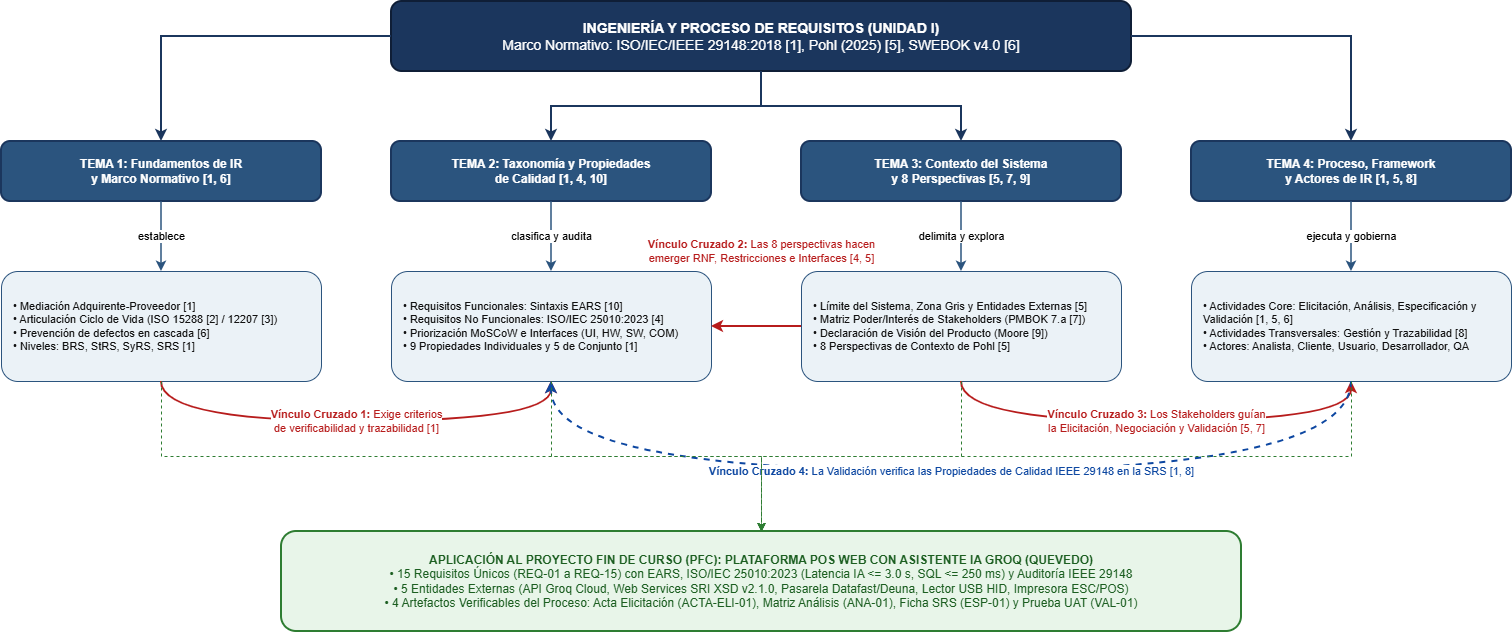
\includegraphics[width=0.98\textwidth]{figura/mapa_conceptual.png}
	\caption{Mapa Conceptual Integrador de los Cuatro Temas de la Unidad I con Vínculos Cruzados y Aplicación al PFC.}
	\label{fig:mapa_conceptual}
\end{figure}
\subsection{Criterio C3: Actores y Framework de Ingeniería de Requisitos Mapeados al PFC}
Para cubrir íntegramente el Criterio C3 de la Rúbrica SGA (\textit{15\% de la nota: Actores del proceso identificados con roles concretos; actividades core y transversales mapeadas al sistema} \cite{ieee29148, pohl2025, ireb2023}), en la Tabla \ref{tab:actores_framework} se relaciona cada actor del proyecto con sus responsabilidades concretas dentro del framework de IR y los artefactos generados para el PFC.
\begin{table}[htbp]
	\centering
	\scriptsize
	\caption{Mapeo de Actores del Proceso y Actividades Core/Transversales del Framework de IR Aplicado al PFC \cite{ieee29148, pohl2025}}
	\label{tab:actores_framework}
	\begin{tabularx}{\textwidth}{>{\raggedright\arraybackslash}p{0.16\textwidth} >{\raggedright\arraybackslash}p{0.16\textwidth} Y Y}
		\toprule
		\textbf{Actor del Proceso de IR} & \textbf{Persona / Entidad en el PFC} & \textbf{Participación en Actividades Core (Elicitación, Análisis, Especificación, Validación)} & \textbf{Participación en Actividades Transversales (Gestión, Trazabilidad y Control de Cambios)} \\
		\midrule
		\textbf{Ingeniero de Requisitos / Analista Líder} & José Ignacio Gilces Carranza (\textit{Analista Líder}) & Diseña y conduce las entrevistas contextuales; aplica las 8 perspectivas de Pohl; redacta formalmente los requisitos en sintaxis EARS e ISO 25010 libres de implementación; ejecuta la verificación de propiedades IEEE 29148. & Administra la línea base de requisitos (\textit{Baseline v1.0}), mantiene la matriz de trazabilidad bidireccional y evalúa el impacto de las solicitudes de cambio. \\
		\midrule
		\textbf{Ingenieros de Requisitos / Investigadores} & Jostin Vélez Vinces y Jeanpierre Robinson Espinoza & Modelan el límite del sistema y sus 5 interfaces externas; construyen el mapa conceptual y prototipos de interfaz; documentan los escenarios de contingencia del módulo de IA y del SRI. & Gestionan la biblioteca de fuentes primarias (estilo IEEE) y aseguran la consistencia terminológica del glosario de dominio eléctrico. \\
		\midrule
		\textbf{Cliente / Patrocinador (\textit{Sponsor})} & Propietario del Almacén Eléctrico (SH-03) & Define los objetivos estratégicos de negocio (reducción de atención a $\le 60\text{ s}$); establece las restricciones de presupuesto operativo; aprueba la Declaración de Visión en formato Moore. & Autoriza o rechaza solicitudes de cambio de alcance (\textit{Change Requests}) que impacten los costos o plazos acordados. \\
		\midrule
		\textbf{Usuarios Operativos y Tácticos} & Cajeros de Mostrador (SH-01) y Administrador (SH-02) & Aportan el conocimiento empírico del dominio durante la observación en sitio; detallan la jerga eléctrica local; participan en las sesiones de validación de usabilidad y navegación por teclado (F1--F12). & Reportan necesidades operativas adicionales o casos de productos eléctricos especiales durante las revisiones iterativas. \\
		\midrule
		\textbf{Arquitecto y Desarrolladores de Software} & Equipo Técnico de Construcción Posterior & Analizan la factibilidad técnica (propiedad IEEE 29148) de los umbrales de desempeño exigidos ($\le 3.0\text{ s}$ en recomendaciones IA y $\le 250\text{ ms}$ en búsquedas locales) sin contaminar la SRS con diseño prematuro. & Utilizan los identificadores únicos (\texttt{REQ-01} a \texttt{REQ-15}) para trazar futuramente los módulos de arquitectura y casos de prueba de verificación. \\
		\midrule
		\textbf{Auditor / Ente Regulador} & Contador / Servicio de Rentas Internas (SH-05) & Provee las fichas técnicas normativas de comprobantes electrónicos y las restricciones legales de auditoría tributaria y protección de datos personales (LOPDP). & Audita la trazabilidad regulatoria ante reformas fiscales o actualizaciones de porcentajes impositivos en el Ecuador. \\
		\bottomrule
	\end{tabularx}
\end{table}
\subsection{Criterio C4: Aplicación Práctica de la Secuencia del Proceso de Requisitos (Artefactos Parciales del PFC)}
En cumplimiento del Criterio C4 de la Rúbrica SGA (\textit{25\% de la nota: Se muestra la secuencia de actividades del proceso —elicitación, análisis, especificación, validación— con artefactos parciales para el sistema seleccionado} \cite{ieee29148, pohl2025}), a continuación se documenta la trazabilidad secuencial completa de cómo una necesidad real del almacén eléctrico fue procesada a través de las cuatro fases del proceso de ingeniería de requisitos mediante artefactos verificables y libres de tecnologías de diseño.
\subsubsection{Fase 1: Artefacto Parcial de Elicitación (Ficha de Entrevista Contextual y Observación en Sitio)}
Se aplicó la técnica combinada de \textbf{Entrevista Semiestructurada} y \textbf{Observación Directa (\textit{Shadowing})} en un local de materiales eléctricos de Quevedo \cite{pohl2025, wiegers2013}.
\begin{table}[htbp]
	\centering
	\scriptsize
	\caption{Artefacto de Elicitación ELI-01: Registro de Entrevista y Observación en Mostrador}
	\label{tab:artefacto_elicitacion}
	\begin{tabularx}{\textwidth}{>{\raggedright\arraybackslash}p{0.22\textwidth} Y}
		\toprule
		\textbf{Campo del Artefacto} & \textbf{Registro de Evidencia Empírica en el Contexto Local (Quevedo)} \\
		\midrule
		\textbf{Código y Fecha:} & \texttt{ACTA-ELI-01} $\cdot$ Fecha de levantamiento: 06 de noviembre de 2026 $\cdot$ Duración: 45 minutos. \\
		\textbf{Stakeholders Entrevistados:} & SH-01 (Cajero principal de mostrador) y SH-02 (Administrador de inventario). \\
		\textbf{Hallazgo de Observación (\textit{As-Is}):} & Se cronometraron 15 atenciones en hora pico (10h30--11h30). Cuando un cliente solicitó un ``contactor trifásico de 25A bobina 220V'' cuya marca habitual estaba agotada, el cajero tardó \textbf{4 minutos y 15 segundos} revisando cajas físicamente en percha y llamando al administrador, provocando que 2 clientes en fila abandonaran el local. \\
		\textbf{Declaración Textual del Usuario:} & \textit{``Yo sé cobrar rápido cuando me traen el código exacto, pero cuando me piden un reemplazo eléctrico o no hay stock de una marca, no sé qué otro modelo soporta el mismo amperaje y pierdo mucho tiempo buscando''} (SH-01). \\
		\textbf{Necesidades Brutas Identificadas:} & (N1) Conocer al instante qué producto disponible en bodega sirve como reemplazo técnico seguro; (N2) No depender del ratón al facturar; (N3) Que la facturación no se detenga si el internet externo presenta intermitencias. \\
		\bottomrule
	\end{tabularx}
\end{table}
\subsubsection{Fase 2: Artefacto Parcial de Análisis y Negociación (Resolución de Conflictos y Matriz de Riesgos)}
Las necesidades brutas elicitadas fueron sometidas a análisis de factibilidad, detección de conflictos entre stakeholders y negociación de acuerdos de requerimientos \cite{swebok2024, ireb2023}:
\begin{table}[htbp]
	\centering
	\scriptsize
	\caption{Artefacto de Análisis ANA-01: Matriz de Negociación de Conflictos y Mitigación de Riesgos}
	\label{tab:artefacto_analisis}
	\begin{tabularx}{\textwidth}{l Y Y Y}
		\toprule
		\textbf{ID Conflicto} & \textbf{Tensión Detectada entre Stakeholders} & \textbf{Análisis de Riesgo Operativo / Económico} & \textbf{Acuerdo de Negociación y Requisito Derivado} \\
		\midrule
		\textbf{CONF-01} & \textbf{SH-01 (Cajero)} solicita un asistente de IA de consulta libre vs. \textbf{SH-02 (Administrador)} exige que jamás se recomiende un artículo agotado o con especificaciones eléctricas inexactas (\textit{alucinación}). & Una consulta abierta sin restricción de inventario puede sugerir marcas que el local no comercializa o capacidades eléctricas inadecuadas, generando reclamos y pérdida de tiempo. & \textbf{Acuerdo:} Especificar que el módulo de recomendación filtre exclusivamente artículos registrados en el catálogo local con saldo disponible $> 0$ y atributos técnicos verificados (deriva en \texttt{REQ-04} y \texttt{REQ-06}). \\
		\midrule
		\textbf{CONF-02} & \textbf{SH-03 (Propietario)} exige no adquirir equipos de cómputo especializados costosos para las cajas vs. \textbf{SH-01 (Cajero)} requiere respuestas de recomendación en $\le 3.0\text{ segundos}$. & El procesamiento pesado en terminales básicas de mostrador degradaría el tiempo de respuesta por encima de los 15 segundos, entorpeciendo la fila de atención. & \textbf{Acuerdo:} Consumir un servicio externo de inferencia de IA de baja latencia mediante interfaz de comunicaciones segura y almacenar temporalmente las consultas frecuentes del día (deriva en \texttt{REQ-08} y \texttt{REQ-14}). \\
		\midrule
		\textbf{CONF-03} & \textbf{Dependencia de servicios externos (IA / SRI)} vs. \textbf{Continuidad de ventas en Quevedo} ante microcortes de conectividad. & Si un servicio externo demora en responder y bloquea la pantalla de cobro, la atención del local quedaría paralizada en hora pico. & \textbf{Acuerdo:} Establecer un límite de espera máximo de $3.0\text{ s}$ con conmutación automática a búsqueda local por subcategoría eléctrica en $\le 200\text{ ms}$ sin interrumpir la facturación (deriva en \texttt{REQ-10}). \\
		\bottomrule
	\end{tabularx}
\end{table}
\subsubsection{Fase 3: Artefacto Parcial de Especificación Detallada (Ficha Técnica de Requisito Crítico SRS)}
Como producto de la fase de especificación conforme a ISO/IEC/IEEE 29148:2018 \cite{ieee29148} y EARS \cite{mavin2009ears}, se documenta la ficha estructurada del requisito crítico \texttt{REQ-04} libre de detalles de implementación:
\begin{table}[htbp]
	\centering
	\scriptsize
	\caption{Artefacto de Especificación ESP-01: Plantilla Detallada IEEE 29148 para el Requisito Crítico REQ-04}
	\label{tab:artefacto_especificacion}
	\begin{tabularx}{\textwidth}{>{\raggedright\arraybackslash}p{0.24\textwidth} Y}
		\toprule
		\textbf{Atributo SRS (IEEE 29148)} & \textbf{Especificación Formal del Artefacto (Agnóstica a la Tecnología)} \\
		\midrule
		\textbf{Identificador y Título:} & \texttt{REQ-04} --- Recomendación Técnica de Suministros Eléctricos Compatibles Acotada a Existencias Reales. \\
		\textbf{Tipo y Prioridad MoSCoW:} & Requisito Funcional de Software (RF) $\cdot$ Prioridad: \textbf{Must Have} (Crítico para el sistema). \\
		\textbf{Declaración EARS (\textit{Event-Driven}):} & \textbf{WHEN} el cajero ingresa un artículo agotado o una consulta electrotécnica en el asistente de ventas (tecla \texttt{F4}), \textit{the Sales Platform shall} consultar al módulo de recomendación de IA filtrando únicamente el catálogo local con saldo disponible mayor a cero y presentar exactamente 3 productos compatibles indicando nombre, tensión/corriente nominal, precio unitario y existencias actuales. \\
		\textbf{Precondiciones Operativas:} & 1. El cajero cuenta con una sesión autenticada y activa en su turno (\texttt{REQ-11}). 2. El catálogo de suministros eléctricos dispone de fichas con parámetros nominales registrados. \\
		\textbf{Estímulo de Entrada:} & Expresión de búsqueda técnica (ej. \textit{``Reemplazo para interruptor riel DIN 2 polos 32A curva C''}) o selección de un artículo con saldo de inventario igual a cero. \\
		\textbf{Reglas de Negocio Asociadas:} & 1. Solo pueden incluirse como candidatos aquellos artículos de la misma familia eléctrica cuyo saldo disponible sea mayor a cero. 2. La consulta enviada al servicio externo no contendrá ningún dato personal del comprador (\texttt{REQ-15}). \\
		\textbf{Postcondiciones / Salida:} & Se despliega en la vista de facturación una lista seleccionable con las 3 opciones en $\le 3.0\text{ s}$ (\texttt{REQ-08}); al confirmar una opción mediante teclado, el artículo se incorpora inmediatamente al detalle de la venta (\texttt{REQ-05}). \\
		\textbf{Trazabilidad Bidireccional:} & \textbf{Origen hacia atrás:} \texttt{ACTA-ELI-01} (SH-01, SH-02) y acuerdo \texttt{CONF-01}. $\rightarrow$ \textbf{Trazabilidad hacia adelante:} Subsistema de Recomendación Técnica y Protocolo de Aceptación \texttt{VAL-UAT-04}. \\
		\bottomrule
	\end{tabularx}
\end{table}
\subsubsection{Fase 4: Artefacto Parcial de Validación y Verificación (Checklist de Inspección y Caso de Prueba de Aceptación)}
Finalmente, en la fase de validación y verificación \cite{ieee29148, pohl2025}, el requisito especificado se somete a un protocolo de prueba de aceptación de usuario (\textit{UAT}) acordado con los stakeholders:
\begin{table}[htbp]
	\centering
	\scriptsize
	\caption{Artefacto de Validación VAL-01: Protocolo de Prueba de Aceptación y Verificación para REQ-04 y REQ-08}
	\label{tab:artefacto_validacion}
	\begin{tabularx}{\textwidth}{>{\raggedright\arraybackslash}p{0.24\textwidth} Y}
		\toprule
		\textbf{Parámetro de Validación} & \textbf{Descripción y Criterio de Aceptación Cuantitativo} \\
		\midrule
		\textbf{ID Caso de Prueba y Objetivo:} & \texttt{VAL-UAT-04} --- Validar la precisión electrotécnica, el filtro de saldo disponible y el tiempo máximo de respuesta del módulo de recomendación en escenario real de mostrador. \\
		\textbf{Escenario y Datos de Entrada:} & Artículo solicitado: \textit{Contactor Trifásico 25A Bobina 220V} (registrado con saldo disponible $= 0$ en inventario). En el catálogo local existen 4 contactores alternativos de 25A/220V con existencias disponibles ($> 5$ unidades) y 2 contactores de 9A (incompatibles por subdimensionamiento eléctrico). \\
		\textbf{Resultado Esperado (Oráculo):} & 1. La Plataforma de Ventas impide facturar el artículo sin existencias (\texttt{REQ-06}). \newline
		2. En un tiempo $\le 3.0\text{ segundos}$ (\texttt{REQ-08}), el sistema presenta en pantalla 3 alternativas de 25A/220V con existencias reales y \textbf{excluye} los contactores de 9A por no soportar la corriente nominal requerida. \\
		\textbf{Verificación IEEE 29148:} & [$\checkmark$] ¿Es verificable cuantitativamente? Sí ($\le 3.0\text{ s}$, exactamente 3 ítems, saldo $>0$). \newline
		[$\checkmark$] ¿Es apropiado al nivel (libre de tecnologías de diseño)? Sí, especifica capacidades puras de dominio. \newline
		[$\checkmark$] ¿Validado por el usuario operativo (SH-01) y administrador (SH-02)? \textbf{CONFORME / APROBADO}. \\
		\bottomrule
	\end{tabularx}
\end{table}
